\chapter{PENGUJIAN DAN ANALISIS}
\label{chap:pengujiananalisis}

% Ubah bagian-bagian berikut dengan isi dari pengujian dan analisis

Pada bab ini, akan dijelaskan mengenai hasil pengujian dan pembahasan dari penelitian yang telah diuraikan pada metodologi. Selain itu, akan dipaparkan juga mengenai skenario pengujian yang dilakukan untuk mengevaluasi performa sistem secara keseluruhan. Pengujian ini dilakukan dengan tujuan untuk memastikan bahwa sistem yang dirancang mampu berfungsi dengan baik dalam berbagai kondisi dan situasi yang mungkin dihadapi dalam penggunaannya.

\section{Skenario Pengujian}
\label{sec:skenariopengujian}

Pengujian dilakukan untuk mengetahui performa model dalam melakukan deteksi dan mengikuti objek oleh kursi roda otonom. Skenario pengujian ini dirancang untuk mengukur berbagai aspek dari sistem, termasuk akurasi deteksi, kecepatan pemrosesan, respons sistem terhadap objek, dan tingkat keberhasilan mengidentifikasi tracking. Skenario pengujian yang akan dilakukan adalah sebagai berikut:

\begin{enumerate}
    \item Hasil Pengujian Performa Model
    \item Pengujian Berdasarkan FPS
    \item Pengujian Berdasarkan Hasil Response Time
    \item Pengujian Keberhasilan Tracking
    \item Pengujian Tingkat Pencahayaan
    \item Pengujian Kesesuaian Jarak Deteksi
    \item Performa Pergerakan Mengikuti Objek
    \item Performa Keberhasilan Mengikuti Objek
\end{enumerate}

\newpage
\section{Hasil Pengujian Performa Menggunakan Confusion Matrix}
\label{sec:hasilperformaconfisionMatrix}

Sebanyak 15163 citra manusia dan 590 data validasi digunakan sebagai data latih awal. Melalui proses augmentasi, jumlah data latih meningkat menjadi 4.359, sementara data validasi bertambah menjadi 1.023. Setelah jumlah dataset ditentukan, langkah selanjutnya adalah membuat API key pada Roboflow yang kemudian diintegrasikan untuk proses pelatihan model.

Proses pelatihan model dimulai setelah seluruh dataset dimuat. Selama pelatihan, beberapa parameter digunakan dan hasilnya dibandingkan menggunakan nilai confusion matrix serta metrik akurasi deteksi seperti mAP score, precision, dan box loss. Layer input pertama dijelaskan sebagai tahap awal pelatihan model.

Pelatihan dilakukan selama 100 epoch pertama dengan ukuran batch sebesar 16 piksel, dan data diubah ukurannya menjadi 800 x 800 piksel selama preprocessing. Tujuan dari pelatihan ini adalah untuk mengevaluasi seberapa besar peningkatan performa model terlatih sebelumnya dalam mendeteksi manusia berdasarkan jumlah epoch yang dilakukan. Pada akhir 100 epoch, nilai box loss yang dihasilkan adalah 0,82978, yang menunjukkan kemampuan model untuk memprediksi bounding box dengan baik di sekitar objek. Penurunan nilai box loss selama pelatihan menunjukkan bahwa model berhasil belajar mengidentifikasi koordinat bounding box secara akurat.

Selama validasi, nilai box loss tercatat sebesar 1,199, yang mengindikasikan kemampuan model dalam mengenali objek pada data uji. Penurunan box loss pada tahap validasi mencerminkan kemampuan model untuk mendeteksi objek secara general, tidak hanya pada data latih. Nilai mAP score divisualisasikan pada Gambar, dengan hasil skor mAP sebesar 81,85% untuk IoU minimum 0,5, yang menegaskan akurasi tinggi dalam mendeteksi objek.

Secara keseluruhan, hasil pelatihan model dirangkum pada Gambar. Nilai box loss pada pelatihan adalah 0,82978, nilai cls loss adalah 0,57615, dan dfl loss sebesar 1,1197. Metrik lainnya meliputi precision (0,84974), recall (0,72608), mAP50 (0,81855), dan mAP50-95 (0,53527). Selama validasi, nilai box loss tercatat sebesar 1,199, cls loss sebesar 0,86314, dan dfl loss sebesar 1,4956.

Visualisasi hasil model disajikan melalui confusion matrix yang menggambarkan kinerja deteksi secara rinci. Matrix ini menunjukkan 1.806 data sebagai True Positive (manusia terdeteksi dengan benar), 483 data sebagai False Positive (objek salah terdeteksi sebagai manusia), dan 475 data sebagai False Negative (manusia yang tidak terdeteksi).

Kurva F1-Confidence yang dihasilkan selama pelatihan menunjukkan hubungan antara confidence score dan F1-score. Model mencapai nilai F1-score tertinggi sebesar 0,78 pada confidence score 0,450, mengindikasikan keseimbangan optimal antara precision dan recall. Namun, kurva menunjukkan penurunan signifikan setelah confidence score mencapai sekitar 0,8, yang menandakan bahwa pada tingkat confidence yang sangat tinggi, model cenderung mengabaikan banyak true positives, sehingga menurunkan F1-score keseluruhan.

Inferensi terhadap data uji juga dilakukan menggunakan model yang telah dilatih. Hasilnya menunjukkan tingkat confidence yang tinggi pada deteksi objek manusia, sebagaimana divisualisasikan dalam gambar hasil pengujian

\section{Pengujian Berdasarkan FPS}
\label{sec:pengujianberdasarkanfps}

Pengujian ini dilakukan untuk menganalisis kecepatan pemrosesan sistem dalam satuan Frame per Second (FPS). FPS yang tinggi menunjukkan bahwa sistem dapat bekerja dengan baik secara real-time. Grafik hasil pengujian disertakan untuk memudahkan visualisasi performa.

\section{Pengujian Berdasarkan Response Time}
\label{sec:pengujianberdasarkanresponsetime}

Bagian ini mengukur waktu yang dibutuhkan sistem untuk merespons setiap perubahan lingkungan atau perintah yang diterima. Response Time sangat penting untuk mengukur responsivitas sistem dalam skenario dinamis.

\section{Pengujian Keberhasilan Tracking}
\label{sec:pengujiankeberhasiltracking}

Bagian ini mengevaluasi keberhasilan sistem dalam melakukan tracking terhadap objek target. Tingkat keberhasilan dianalisis untuk mengetahui keandalan sistem dalam berbagai skenario.

\section{Pengujian Tingkat Pencahayaan}
\label{sec:pengujiantingkatpencahayaan}

Pengujian dilakukan untuk mengukur kemampuan sistem dalam mendeteksi objek pada berbagai tingkat pencahayaan. Fokus pengujian ini adalah memastikan bahwa sistem dapat berfungsi dengan baik dalam kondisi pencahayaan yang berbeda.

\newpage
\section{Pengujian Kesesuaian Jarak Deteksi}
\label{sec:pengujiankesesuaianjarakdeteksi}

Pengujian dilakukan untuk mengukur kemampuan sistem dalam mendeteksi objek pada berbagai jarak dan menganalisis performa sistem pada jarak-jarak tersebut. Fokus pengujian ini adalah memastikan bahwa ketika objek berada pada jarak yang sangat dekat (\textless 1m), sistem mengirimkan kode instruksi untuk berhenti (diam) guna mencegah tabrakan.

\begin{table}[H]
    \centering
    \caption{Data Jarak (\textless 1m) untuk Diam}
    \label{tab:jarak_diam}
    \begin{tabular}{|c|c|c|c|c|c|c|c|c|}
    \hline
    Waktu & Reg (s) & YOLO (m) & MP (m) & x (px) & Deteksi & Terkirim & Keterangan \\ \hline
    12:55:12 & 0.8402 & 2.0631 & 0.9852 & 833 & b'C\textbackslash n' & b'C\textbackslash n' & Stop \\ \hline
    12:55:15 & 0.2585 & 1.1003 & 0.8942 & 242 & b'C\textbackslash n' & b'C\textbackslash n' & Stop \\ \hline
    12:55:24 & 2.1821 & 1.1773 & 0.9652 & 511 & b'C\textbackslash n' & b'C\textbackslash n' & Stop \\ \hline
    12:58:13 & 1.4998 & 1.4123 & 0.9574 & 531 & b'C\textbackslash n' & b'C\textbackslash n' & Stop \\ \hline
    12:58:14 & 0.2538 & 1.4538 & 0.9899 & 555 & b'C\textbackslash n' & b'C\textbackslash n' & Stop \\ \hline
    12:58:19 & 2.4033 & 1.1691 & 0.9213 & 852 & b'C\textbackslash n' & b'C\textbackslash n' & Stop \\ \hline
    12:58:19 & 0.4079 & 1.1839 & 0.9118 & 854 & b'C\textbackslash n' & b'C\textbackslash n' & Stop \\ \hline
    12:58:20 & 0.8708 & 1.0960 & 0.9548 & 528 & b'C\textbackslash n' & b'C\textbackslash n' & Stop \\ \hline
    12:58:21 & 0.4262 & 1.1003 & 0.9189 & 547 & b'C\textbackslash n' & b'C\textbackslash n' & Stop \\ \hline
    12:58:21 & 0.3497 & 1.1032 & 0.8985 & 554 & b'C\textbackslash n' & b'C\textbackslash n' & Stop \\ \hline
    12:58:21 & 0.3314 & 1.1032 & 0.8785 & 518 & b'C\textbackslash n' & b'C\textbackslash n' & Stop \\ \hline
    13:00:57 & 1.4848 & 1.1594 & 0.9943 & 208 & b'C\textbackslash n' & b'C\textbackslash n' & Stop \\ \hline
    13:01:15 & 1.5987 & 1.3643 & 0.9899 & 849 & b'C\textbackslash n' & b'C\textbackslash n' & Stop \\ \hline
    13:01:19 & 0.2719 & 1.0989 & 0.7700 & 856 & b'C\textbackslash n' & b'C\textbackslash n' & Stop \\ \hline
    13:01:19 & 0.2509 & 1.1452 & 0.5782 & 856 & b'C\textbackslash n' & b'C\textbackslash n' & Stop \\ \hline
    17:41:34 & 0.3036 & 1.4339 & 0.9447 & 647 & b'C\textbackslash n' & b'C\textbackslash n' & Stop \\ \hline
    17:41:35 & 0.3326 & 1.4291 & 0.8357 & 642 & b'C\textbackslash n' & b'C\textbackslash n' & Stop \\ \hline
    17:41:36 & 0.3588 & 1.4389 & 0.8222 & 672 & b'C\textbackslash n' & b'C\textbackslash n' & Stop \\ \hline
    17:41:45 & 0.3092 & 1.3913 & 0.7249 & 640 & b'C\textbackslash n' & b'C\textbackslash n' & Stop \\ \hline
    17:42:04 & 15.5192 & 1.4563 & 0.5955 & 213 & b'C\textbackslash n' & b'C\textbackslash n' & Stop \\ \hline
    \end{tabular}
    \end{table}

Tabel \ref{tab:jarak_diam} menunjukkan data jarak yang diukur ketika objek berada pada jarak kurang dari 1 meter. Data ini mencakup waktu deteksi, jarak deteksi dari YOLOv11 dan MediaPipe Pose, posisi objek dalam frame, hasil deteksi, instruksi yang dikirimkan, dan keterangan mengenai status objek. Data ini memberikan gambaran kinerja sistem dalam mengikuti objek yang berada pada jarak dekat, termasuk kecepatan respons, akurasi deteksi, dan ketepatan instruksi yang dikirimkan.

Pengujian jarak juga telah diverifikasi secara fisik dengan pengukuran dan perbandingan yang cermat sebelum menyajikan data. Hal ini memastikan akurasi dan keandalan pengukuran jarak yang digunakan dalam evaluasi. Proses verifikasi melibatkan penggunaan alat ukur yang terkalibrasi dan uji coba berulang untuk meminimalkan kesalahan.

\newpage
\section{Performa Pergerakan Mengikuti Objek}
\label{sec:performaakurasiobjek}

Analisis dilakukan untuk mengukur seberapa akurat sistem dapat mengikuti objek target, termasuk mempertahankan jarak yang tepat dan tidak kehilangan objek dalam berbagai kondisi.

\subsection{Percobaan Dalam Frame}
\label{subsec:percobaandalamframe}

Bagian ini membahas kemampuan sistem dalam mengikuti objek yang berada di dalam frame kamera dengan fokus utama pada evaluasi kinerja regulator. Tujuannya adalah memastikan bahwa sistem dapat merespons hasil deteksi dengan akurat dan konsisten, sesuai dengan kondisi objek yang terdeteksi di dalam frame kamera. Analisis dilakukan menggunakan 100 data sampel untuk memberikan gambaran kinerja sistem secara menyeluruh.

\begin{longtable}{|c|c|c|c|c|c|c|c|}
    \caption{Data Status Frame (Dalam Frame)} \label{tab:status_dalam_frame} \\
    \hline
    Waktu & Reg (s) & YOLO (m) & MP (m) & x (px) & Deteksi & Terkirim & Keterangan \\ \hline
    \endhead
    \hline \multicolumn{8}{|r|}{Lanjutan ke halaman berikutnya} \\ \hline
    \endfoot
    \endlastfoot
    12:48:09 & 0.2960 & 2.4469 & 2.6214 & 765 & b'E\textbackslash n' & b'C\textbackslash n' & Turn Right \\ \hline
12:48:09 & 0.2991 & 5.6875 & 4.1146 & 484 & b'B\textbackslash n' & b'E\textbackslash n' & Forward \\ \hline
12:48:10 & 0.2516 & 2.2093 & 2.6063 & 595 & b'B\textbackslash n' & b'C\textbackslash n' & Forward \\ \hline
12:48:14 & 2.7739 & 1.4513 & 1.7409 & 128 & b'A\textbackslash n' & b'A\textbackslash n' & Turn Left \\ \hline
12:48:17 & 2.6621 & 1.7109 & 1.1479 & 447 & b'B\textbackslash n' & b'C\textbackslash n' & Forward \\ \hline
12:50:45 & 0.5046 & 2.5900 & 1.4523 & 391 & b'B\textbackslash n' & b'B\textbackslash n' & Forward \\ \hline
12:50:48 & 2.7333 & 1.1421 & 1.9733 & 164 & b'A\textbackslash n' & b'C\textbackslash n' & Turn Left \\ \hline
12:50:51 & 0.4610 & 1.4219 & 1.0142 & 830 & b'E\textbackslash n' & b'E\textbackslash n' & Turn Right \\ \hline
12:50:54 & 2.5388 & 1.4768 & 1.1208 & 501 & b'B\textbackslash n' & b'C\textbackslash n' & Forward \\ \hline
12:50:57 & 0.2675 & 2.0939 & 1.4524 & 825 & b'E\textbackslash n' & b'E\textbackslash n' & Turn Right \\ \hline
12:51:00 & 0.3556 & 1.7144 & 1.5984 & 492 & b'B\textbackslash n' & b'C\textbackslash n' & Forward \\ \hline
12:51:00 & 0.3290 & 1.4978 & 1.4964 & 466 & b'B\textbackslash n' & b'B\textbackslash n' & Forward \\ \hline
12:51:07 & 3.9922 & 1.7796 & 1.3830 & 896 & b'E\textbackslash n' & b'C\textbackslash n' & Turn Right \\ \hline
12:51:08 & 0.3129 & 1.6801 & 1.7017 & 525 & b'B\textbackslash n' & b'C\textbackslash n' & Forward \\ \hline
12:51:09 & 0.3226 & 1.6408 & 1.7256 & 463 & b'B\textbackslash n' & b'B\textbackslash n' & Forward \\ \hline
12:51:11 & 2.3641 & 1.5332 & 1.1242 & 850 & b'E\textbackslash n' & b'C\textbackslash n' & Turn Right \\ \hline
12:51:17 & 5.5467 & 2.2628 & 1.6525 & 563 & b'B\textbackslash n' & b'C\textbackslash n' & Forward \\ \hline
12:51:17 & 0.3035 & 1.9853 & 1.6709 & 408 & b'B\textbackslash n' & b'B\textbackslash n' & Forward \\ \hline
12:51:18 & 0.3176 & 1.6668 & 1.5184 & 189 & b'A\textbackslash n' & b'C\textbackslash n' & Turn Left \\ \hline
12:51:18 & 0.3818 & 1.5277 & 1.4295 & 202 & b'A\textbackslash n' & b'A\textbackslash n' & Turn Left \\ \hline
12:51:21 & 2.9916 & 2.0186 & 1.6728 & 440 & b'B\textbackslash n' & b'C\textbackslash n' & Forward \\ \hline
12:51:21 & 0.3446 & 2.4830 & 1.6701 & 601 & b'B\textbackslash n' & b'B\textbackslash n' & Forward \\ \hline
12:51:22 & 0.2721 & 2.6141 & 1.7926 & 769 & b'E\textbackslash n' & b'C\textbackslash n' & Turn Right \\ \hline
12:51:22 & 0.2947 & 2.7330 & 1.5570 & 867 & b'E\textbackslash n' & b'E\textbackslash n' & Turn Right \\ \hline
12:51:26 & 3.8579 & 2.5354 & 1.6134 & 553 & b'B\textbackslash n' & b'C\textbackslash n' & Forward \\ \hline
12:51:26 & 0.4472 & 1.9174 & 1.2873 & 212 & b'A\textbackslash n' & b'C\textbackslash n' & Turn Left \\ \hline
12:51:27 & 0.2536 & 1.6668 & 1.9112 & 142 & b'A\textbackslash n' & b'A\textbackslash n' & Turn Left \\ \hline
12:51:30 & 3.3993 & 2.4258 & 1.4468 & 551 & b'B\textbackslash n' & b'C\textbackslash n' & Forward \\ \hline
12:51:36 & 4.6957 & 1.7144 & 1.8941 & 478 & b'B\textbackslash n' & b'B\textbackslash n' & Forward \\ \hline
12:51:37 & 1.7377 & 1.5194 & 1.8537 & 182 & b'A\textbackslash n' & b'C\textbackslash n' & Turn Left \\ \hline
12:51:42 & 0.2820 & 1.4820 & 1.5157 & 424 & b'B\textbackslash n' & b'C\textbackslash n' & Forward \\ \hline
12:51:42 & 0.2867 & 1.5473 & 1.6206 & 481 & b'B\textbackslash n' & b'B\textbackslash n' & Forward \\ \hline
12:51:44 & 0.3591 & 2.1528 & 1.7878 & 245 & b'A\textbackslash n' & b'C\textbackslash n' & Turn Left \\ \hline
12:51:44 & 0.2619 & 1.6003 & 1.9633 & 426 & b'B\textbackslash n' & b'A\textbackslash n' & Forward \\ \hline
12:51:45 & 0.2692 & 1.5704 & 1.6022 & 449 & b'B\textbackslash n' & b'C\textbackslash n' & Forward \\ \hline
12:51:45 & 0.3616 & 1.8259 & 1.5129 & 249 & b'A\textbackslash n' & b'B\textbackslash n' & Turn Left \\ \hline
12:51:48 & 2.8133 & 1.7721 & 1.1400 & 766 & b'E\textbackslash n' & b'C\textbackslash n' & Turn Right \\ \hline
12:51:48 & 0.2701 & 1.9485 & 1.8638 & 792 & b'E\textbackslash n' & b'E\textbackslash n' & Turn Right \\ \hline
12:51:51 & 2.5508 & 2.2628 & 1.9379 & 569 & b'B\textbackslash n' & b'C\textbackslash n' & Forward \\ \hline
12:51:52 & 0.6972 & 1.9174 & 1.6452 & 394 & b'B\textbackslash n' & b'B\textbackslash n' & Forward \\ \hline
12:51:52 & 0.3755 & 1.5912 & 1.3909 & 185 & b'A\textbackslash n' & b'C\textbackslash n' & Turn Left \\ \hline
12:51:52 & 0.3613 & 1.4716 & 1.2101 & 174 & b'A\textbackslash n' & b'A\textbackslash n' & Turn Left \\ \hline
12:51:55 & 0.3125 & 1.9262 & 1.1721 & 564 & b'B\textbackslash n' & b'C\textbackslash n' & Forward \\ \hline
12:51:56 & 0.3797 & 1.9667 & 1.6343 & 835 & b'E\textbackslash n' & b'B\textbackslash n' & Turn Right \\ \hline
12:51:56 & 0.2506 & 1.9262 & 1.7147 & 880 & b'E\textbackslash n' & b'C\textbackslash n' & Turn Right \\ \hline
12:51:56 & 0.2716 & 1.9759 & 1.6276 & 871 & b'E\textbackslash n' & b'E\textbackslash n' & Turn Right \\ \hline
12:52:05 & 0.2830 & 1.9395 & 1.9075 & 502 & b'B\textbackslash n' & b'C\textbackslash n' & Forward \\ \hline
12:55:09 & 1.9217 & 1.5004 & 1.8914 & 861 & b'E\textbackslash n' & b'E\textbackslash n' & Turn Right \\ \hline
12:55:10 & 0.3128 & 1.4414 & 1.8698 & 858 & b'E\textbackslash n' & b'C\textbackslash n' & Turn Right \\ \hline
12:55:10 & 0.3967 & 1.7356 & 1.0821 & 856 & b'E\textbackslash n' & b'E\textbackslash n' & Turn Right \\ \hline
12:55:13 & 0.3498 & 2.0186 & 1.9290 & 520 & b'B\textbackslash n' & b'C\textbackslash n' & Forward \\ \hline
12:55:14 & 0.3321 & 1.8664 & 1.4010 & 511 & b'B\textbackslash n' & b'B\textbackslash n' & Forward \\ \hline
12:55:15 & 1.6785 & 1.1238 & 1.0672 & 170 & b'A\textbackslash n' & b'C\textbackslash n' & Turn Left \\ \hline
12:55:18 & 0.2536 & 1.2489 & 1.0783 & 483 & b'B\textbackslash n' & b'C\textbackslash n' & Forward \\ \hline
12:55:18 & 0.3224 & 1.2129 & 1.4666 & 168 & b'A\textbackslash n' & b'C\textbackslash n' & Turn Left \\ \hline
12:55:19 & 0.3399 & 1.1515 & 1.3422 & 165 & b'A\textbackslash n' & b'A\textbackslash n' & Turn Left \\ \hline
12:55:22 & 0.3309 & 1.5194 & 1.5842 & 504 & b'B\textbackslash n' & b'C\textbackslash n' & Forward \\ \hline
12:55:22 & 0.3887 & 1.4690 & 1.6042 & 528 & b'B\textbackslash n' & b'B\textbackslash n' & Forward \\ \hline
12:55:25 & 0.4715 & 1.1164 & 1.4924 & 170 & b'A\textbackslash n' & b'C\textbackslash n' & Turn Left \\ \hline
12:55:29 & 1.1263 & 1.4029 & 1.2103 & 509 & b'B\textbackslash n' & b'C\textbackslash n' & Forward \\ \hline
12:55:30 & 0.3296 & 1.4219 & 1.2387 & 508 & b'B\textbackslash n' & b'B\textbackslash n' & Forward \\ \hline
12:58:02 & 1.9436 & 1.2696 & 1.0367 & 149 & b'A\textbackslash n' & b'C\textbackslash n' & Turn Left \\ \hline
12:58:03 & 0.3955 & 1.0975 & 1.0832 & 145 & b'A\textbackslash n' & b'A\textbackslash n' & Turn Left \\ \hline
12:58:03 & 0.3395 & 1.6971 & 1.2674 & 619 & b'B\textbackslash n' & b'C\textbackslash n' & Forward \\ \hline
12:58:03 & 0.2777 & 1.6473 & 1.6845 & 616 & b'B\textbackslash n' & b'B\textbackslash n' & Forward \\ \hline
12:58:04 & 0.3573 & 1.4291 & 1.9911 & 795 & b'E\textbackslash n' & b'C\textbackslash n' & Turn Right \\ \hline
12:58:05 & 0.3560 & 1.6768 & 1.8145 & 795 & b'E\textbackslash n' & b'E\textbackslash n' & Turn Right \\ \hline
12:58:05 & 0.3549 & 1.3890 & 1.6223 & 130 & b'A\textbackslash n' & b'C\textbackslash n' & Turn Left \\ \hline
12:58:05 & 0.4054 & 1.3446 & 1.3906 & 174 & b'A\textbackslash n' & b'A\textbackslash n' & Turn Left \\ \hline
12:58:09 & 1.6364 & 1.4665 & 1.1057 & 425 & b'B\textbackslash n' & b'C\textbackslash n' & Forward \\ \hline
12:58:10 & 1.2931 & 1.4123 & 1.6479 & 320 & b'A\textbackslash n' & b'C\textbackslash n' & Turn Left \\ \hline
12:58:11 & 0.3293 & 1.2094 & 1.7544 & 445 & b'B\textbackslash n' & b'C\textbackslash n' & Forward \\ \hline
12:58:11 & 0.5372 & 1.2008 & 1.7284 & 503 & b'B\textbackslash n' & b'B\textbackslash n' & Forward \\ \hline
12:58:25 & 4.1776 & 1.1047 & 1.2300 & 197 & b'A\textbackslash n' & b'C\textbackslash n' & Turn Left \\ \hline
12:58:26 & 0.6310 & 1.1284 & 1.2368 & 195 & b'A\textbackslash n' & b'A\textbackslash n' & Turn Left \\ \hline
12:58:28 & 2.0228 & 1.3319 & 1.2516 & 442 & b'B\textbackslash n' & b'C\textbackslash n' & Forward \\ \hline
12:58:28 & 0.3156 & 1.3754 & 1.5678 & 432 & b'B\textbackslash n' & b'B\textbackslash n' & Forward \\ \hline
13:00:55 & 1.9408 & 1.0975 & 1.0855 & 185 & b'A\textbackslash n' & b'C\textbackslash n' & Turn Left \\ \hline
13:00:55 & 0.4380 & 1.0975 & 1.1142 & 177 & b'A\textbackslash n' & b'C\textbackslash n' & Turn Left \\ \hline
13:00:56 & 0.3263 & 1.0960 & 1.1078 & 167 & b'A\textbackslash n' & b'A\textbackslash n' & Turn Left \\ \hline
13:00:58 & 0.3332 & 1.3091 & 1.8538 & 444 & b'B\textbackslash n' & b'C\textbackslash n' & Forward \\ \hline
13:00:58 & 0.2737 & 1.6903 & 1.0003 & 215 & b'A\textbackslash n' & b'B\textbackslash n' & Turn Left \\ \hline
13:00:59 & 0.2535 & 1.6869 & 1.4439 & 228 & b'A\textbackslash n' & b'C\textbackslash n' & Turn Left \\ \hline
13:00:59 & 0.3323 & 1.7536 & 1.9650 & 225 & b'A\textbackslash n' & b'A\textbackslash n' & Turn Left \\ \hline
13:00:59 & 0.3355 & 1.4267 & 1.5125 & 456 & b'B\textbackslash n' & b'C\textbackslash n' & Forward \\ \hline
13:01:00 & 0.3113 & 1.2734 & 1.1814 & 173 & b'A\textbackslash n' & b'B\textbackslash n' & Turn Left \\ \hline
13:01:01 & 0.4180 & 1.6188 & 1.0805 & 170 & b'A\textbackslash n' & b'C\textbackslash n' & Turn Left \\ \hline
13:01:02 & 0.2600 & 1.5882 & 1.5507 & 222 & b'A\textbackslash n' & b'A\textbackslash n' & Turn Left \\ \hline
13:01:04 & 0.2826 & 1.3173 & 1.3641 & 483 & b'B\textbackslash n' & b'C\textbackslash n' & Forward \\ \hline
13:01:05 & 0.2677 & 1.3256 & 1.3744 & 534 & b'B\textbackslash n' & b'B\textbackslash n' & Forward \\ \hline
13:01:07 & 0.2501 & 1.1872 & 1.1742 & 513 & b'B\textbackslash n' & b'C\textbackslash n' & Forward \\ \hline
13:01:08 & 0.3496 & 1.3298 & 1.2935 & 499 & b'B\textbackslash n' & b'B\textbackslash n' & Forward \\ \hline
13:01:08 & 0.4923 & 1.6188 & 1.3519 & 211 & b'A\textbackslash n' & b'C\textbackslash n' & Turn Left \\ \hline
13:01:09 & 0.3287 & 1.7039 & 1.7476 & 202 & b'A\textbackslash n' & b'A\textbackslash n' & Turn Left \\ \hline
13:01:11 & 2.7773 & 1.5305 & 1.8361 & 517 & b'B\textbackslash n' & b'C\textbackslash n' & Forward \\ \hline
13:01:13 & 1.1224 & 1.8459 & 1.5848 & 850 & b'E\textbackslash n' & b'C\textbackslash n' & Turn Right \\ \hline
13:01:13 & 0.2936 & 1.5942 & 1.0293 & 832 & b'E\textbackslash n' & b'E\textbackslash n' & Turn Right \\ \hline
13:01:17 & 0.2969 & 1.1193 & 1.0841 & 540 & b'B\textbackslash n' & b'C\textbackslash n' & Forward \\ \hline
13:01:17 & 0.3835 & 1.1238 & 1.0723 & 862 & b'E\textbackslash n' & b'B\textbackslash n' & Turn Right \\ \hline
13:01:18 & 0.3058 & 1.1253 & 1.0494 & 845 & b'E\textbackslash n' & b'C\textbackslash n' & Turn Right \\ \hline
\end{longtable}

Tabel \ref{tab:status_dalam_frame} menunjukkan data status dalam frame selama pengujian. Data ini mencakup waktu deteksi, jarak deteksi dari YOLOv11 dan MediaPipe Pose, posisi objek dalam frame, hasil deteksi, instruksi yang dikirimkan, dan keterangan mengenai status objek. Data ini memberikan gambaran kinerja sistem dalam mengikuti objek yang berada di dalam frame kamera, termasuk kecepatan respons, akurasi deteksi, dan ketepatan instruksi yang dikirimkan.

Data yang terdapat pada tabel telah diolah dan ditampilkan dalam bentuk plot untuk mempermudah visualisasi hubungan antara waktu dan instruksi yang dikirimkan oleh sistem. Dengan memanfaatkan plot ini, pola serta tren dalam data dapat diamati secara lebih jelas, sehingga memberikan gambaran yang lebih komprehensif mengenai kinerja sistem selama pengujian.

\begin{figure}[H]
    \centering
    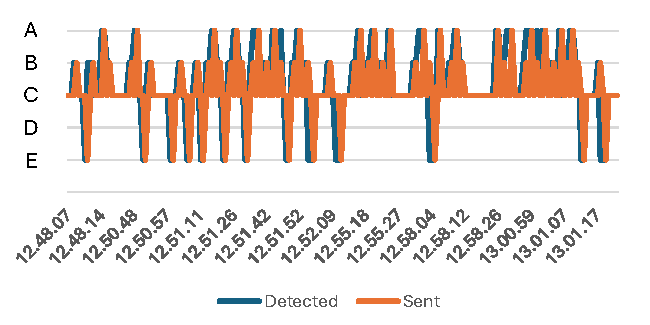
\includegraphics[width=1\textwidth]{gambar/tex/sents.pdf}
    \caption{Detection and Transmission Plots.}
    \label{fig:detection_transmission_plots}
\end{figure}

Visualisasi pada gambar \ref{fig:detection_transmission_plots} berperan penting dalam mendeteksi adanya anomali atau kesalahan yang mungkin terjadi selama proses pengujian. Data yang dipilih untuk divisualisasikan merupakan salah satu hasil terbaik dari serangkaian percobaan terpisah yang telah dilakukan. Hal ini menunjukkan bahwa data tersebut merepresentasikan kondisi sistem yang optimal dan relevan untuk dianalisis lebih lanjut.

\begin{table}[H]
    \centering
    \caption{Summary of Data Transmission and Detection}
    \label{tab:summary_data_transmission_detection}
    \begin{tabular}{|c|c|}
        \hline 
        \cellcolor[HTML]{000000} & \cellcolor[HTML]{C0C0C0} \textbf{Percentage}   \\ \hline
        \cellcolor[HTML]{C0C0C0} \textbf{Transmitted as \texttt{C}} & 55.4  \\ \hline
        \cellcolor[HTML]{C0C0C0} \textbf{Same Register}  & 38.3 \\ \hline
        \cellcolor[HTML]{C0C0C0} \textbf{Different Register}  & 6.3 \\ \hline
    \end{tabular}
\end{table}

Tabel \ref{tab:summary_data_transmission_detection} merangkum data transmisi dan deteksi. Persentase data yang dikirim sebagai \texttt{C} adalah 55.4\%, yang menunjukkan bahwa sistem sering mengirim instruksi untuk berhenti. Persentase data di mana deteksi dan data yang dikirim sama adalah 38.3\%, yang menunjukkan bahwa sistem berjalan sesuai dengan deteksi yang dilakukan. Persentase data di mana deteksi dan data yang dikirim berbeda adalah 6.3\%, yang menunjukkan adanya galat atau kesalahan dalam sistem.

\newpage
\subsection{Percobaan Bergerak Maju}
\label{subsec:percobaanbergerakmaju}

Bagian ini membahas kemampuan sistem dalam mengikuti objek yang bergerak maju dengan kecepatan konstan. Tantangan yang dihadapi adalah bagaimana sistem mempertahankan objek dalam frame sambil melakukan penyesuaian kecepatan yang diperlukan. Solusinya meliputi pemanfaatan fusi data dari YOLOv11 dan MediaPipe Pose, serta penerapan algoritma kontrol yang mampu melakukan koreksi arah tepat waktu, sehingga sistem dapat mengikuti objek yang bergerak maju dengan stabil dan akurat.

\begin{table}[H]
    \centering
    \caption{Data Performa Bergerak Maju}
    \label{tab:performa_bergerak_maju}
    \begin{tabular}{|c|c|c|c|c|c|c|c|}
    \hline
    Waktu & Reg (s) & YOLO (m) & MP (m) & x (px) & Deteksi & Terkirim & Keterangan \\ \hline
    12.48.09 & 0.2991 & 5.6875 & 46.1146 & 484 & b'B\textbackslash n' & b'E\textbackslash n' & Forward \\ \hline
    12.48.10 & 0.2516 & 2.2093 & 5.6063 & 595 & b'B\textbackslash n' & b'C\textbackslash n' & Forward \\ \hline
    12.48.17 & 2.6621 & 1.7109 & 3.1479 & 447 & b'B\textbackslash n' & b'C\textbackslash n' & Forward \\ \hline
    12.50.45 & 0.5046 & 2.5900 & 5.4523 & 391 & b'B\textbackslash n' & b'C\textbackslash n' & Forward \\ \hline
    12.50.46 & 0.3870 & 2.5980 & 4.9960 & 414 & b'B\textbackslash n' & b'B\textbackslash n' & Forward \\ \hline
    12.50.54 & 2.5388 & 1.4768 & 3.1208 & 501 & b'B\textbackslash n' & b'C\textbackslash n' & Forward \\ \hline
    12.51.00 & 0.3556 & 1.7144 & 1.5984 & 492 & b'B\textbackslash n' & b'C\textbackslash n' & Forward \\ \hline
    12.51.00 & 0.3290 & 1.4978 & 1.4964 & 466 & b'B\textbackslash n' & b'B\textbackslash n' & Forward \\ \hline
    12.51.08 & 0.3129 & 1.6801 & 1.7017 & 525 & b'B\textbackslash n' & b'C\textbackslash n' & Forward \\ \hline
    12.51.09 & 0.3226 & 1.6408 & 1.7256 & 463 & b'B\textbackslash n' & b'B\textbackslash n' & Forward \\ \hline
    12.51.17 & 5.5467 & 2.2628 & 2.6525 & 563 & b'B\textbackslash n' & b'C\textbackslash n' & Forward \\ \hline
    12.51.17 & 0.3035 & 1.9853 & 2.1709 & 408 & b'B\textbackslash n' & b'B\textbackslash n' & Forward \\ \hline
    12.51.21 & 2.9916 & 2.0186 & 3.1728 & 440 & b'B\textbackslash n' & b'C\textbackslash n' & Forward \\ \hline
    12.51.21 & 0.3446 & 2.4830 & 3.1701 & 601 & b'B\textbackslash n' & b'B\textbackslash n' & Forward \\ \hline
    12.51.26 & 3.8579 & 2.5354 & 2.0134 & 553 & b'B\textbackslash n' & b'C\textbackslash n' & Forward \\ \hline
    12.51.30 & 3.3993 & 2.4258 & 2.4468 & 551 & b'B\textbackslash n' & b'C\textbackslash n' & Forward \\ \hline
    12.51.36 & 4.6957 & 1.7144 & 1.8941 & 478 & b'B\textbackslash n' & b'C\textbackslash n' & Forward \\ \hline
    12.51.42 & 0.2820 & 1.4820 & 2.5157 & 424 & b'B\textbackslash n' & b'C\textbackslash n' & Forward \\ \hline
    12.51.42 & 0.2867 & 1.5473 & 1.6206 & 481 & b'B\textbackslash n' & b'B\textbackslash n' & Forward \\ \hline
    12.51.44 & 0.2619 & 1.6003 & 1.9633 & 426 & b'B\textbackslash n' & b'A\textbackslash n' & Forward \\ \hline
    12.51.45 & 0.2692 & 1.5704 & 1.6022 & 449 & b'B\textbackslash n' & b'C\textbackslash n' & Forward \\ \hline
    12.51.51 & 2.5508 & 2.2628 & 1.8379 & 569 & b'B\textbackslash n' & b'C\textbackslash n' & Forward \\ \hline
    12.51.52 & 0.6972 & 1.9174 & 2.2452 & 394 & b'B\textbackslash n' & b'B\textbackslash n' & Forward \\ \hline
    12.51.55 & 0.3125 & 1.9262 & 2.1721 & 564 & b'B\textbackslash n' & b'C\textbackslash n' & Forward \\ \hline
    12.52.05 & 0.2830 & 1.9395 & 2.9075 & 502 & b'B\textbackslash n' & b'C\textbackslash n' & Forward \\ \hline
    12.55.13 & 0.3498 & 2.0186 & 1.9290 & 520 & b'B\textbackslash n' & b'C\textbackslash n' & Forward \\ \hline
    12.55.14 & 0.3321 & 1.8664 & 2.8010 & 511 & b'B\textbackslash n' & b'B\textbackslash n' & Forward \\ \hline
    12.55.18 & 0.2536 & 1.2489 & 1.0783 & 483 & b'B\textbackslash n' & b'C\textbackslash n' & Forward \\ \hline
    12.55.18 & 0.3409 & 1.2734 & 1.0403 & 522 & b'B\textbackslash n' & b'B\textbackslash n' & Forward \\ \hline
    12.55.22 & 0.3309 & 1.5194 & 3.5842 & 504 & b'B\textbackslash n' & b'C\textbackslash n' & Forward \\ \hline
    \end{tabular}
\end{table}

Tabel \ref{tab:performa_bergerak_maju} menunjukkan data performa sistem saat bergerak maju. Data ini mencakup waktu deteksi, jarak deteksi dari YOLOv11 dan MediaPipe Pose, posisi objek dalam frame, hasil deteksi, instruksi yang dikirimkan, dan keterangan mengenai arah gerak. Data ini memberikan gambaran kinerja sistem dalam mengikuti objek yang bergerak maju, termasuk kecepatan respons, akurasi deteksi, dan ketepatan instruksi yang dikirimkan.

\begin{figure}[H]
    \centering
    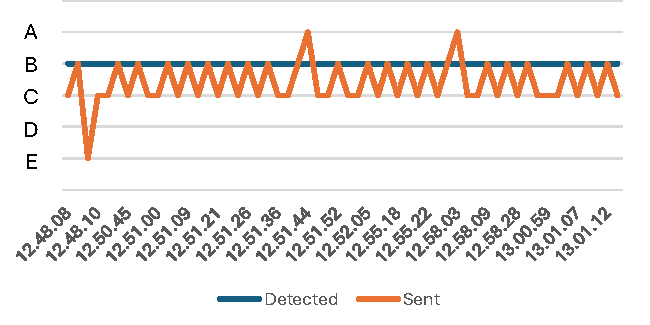
\includegraphics[width=1\textwidth]{gambar/tex/forward.pdf}
    \caption{Straight Movement Plots}
    \label{fig:straight_movement_plots}
\end{figure}

Visualisasi pada gambar \ref{fig:straight_movement_plots} berperan penting dalam mendeteksi adanya anomali atau kesalahan yang mungkin terjadi selama proses pengujian. Data yang dipilih untuk divisualisasikan merupakan salah satu hasil terbaik dari serangkaian percobaan terpisah yang telah dilakukan. Hal ini menunjukkan bahwa data tersebut merepresentasikan kondisi sistem yang optimal dan relevan untuk dianalisis lebih lanjut.

\begin{table}[H]
    \centering
    \caption{Summary of Data During Straight Movement}
    \label{tab:straight_movement_data_transmission_detection}
    \begin{tabular}{|c|c|}
        \hline 
        \cellcolor[HTML]{000000} & \cellcolor[HTML]{C0C0C0} \textbf{Percentage}   \\ \hline
        \cellcolor[HTML]{C0C0C0} \textbf{Transmitted as \texttt{C}} & 15.4  \\ \hline
        \cellcolor[HTML]{C0C0C0} \textbf{Same Register}  & 11.0  \\ \hline
        \cellcolor[HTML]{C0C0C0} \textbf{Different Register}   & 1.5  \\ \hline
    \end{tabular}
\end{table}

Tabel \ref{tab:straight_movement_data_transmission_detection} merangkum data transmisi dan deteksi selama gerakan maju. Persentase data yang dikirim sebagai \texttt{C} adalah 15.4\%, yang menunjukkan bahwa sistem sering mengirim instruksi untuk berhenti. Persentase data di mana deteksi dan data yang dikirim sama adalah 11.0\%, yang menunjukkan bahwa sistem berjalan sesuai dengan deteksi yang dilakukan. Persentase data di mana deteksi dan data yang dikirim berbeda adalah 1.5\%, yang menunjukkan adanya galat atau kesalahan dalam sistem.

\newpage
\subsection{Percobaan Belok Kiri}
\label{subsec:percobaanbelokkiri}

Bagian ini membahas kemampuan sistem dalam mengikuti objek saat berbelok ke kiri. Pada kondisi ini, tantangan yang muncul meliputi perubahan posisi relatif yang terjadi lebih cepat, potensi kehilangan objek dari frame, serta perlunya adaptasi kecepatan motor penggerak. Solusi yang diterapkan adalah penyesuaian parameter kontrol, algoritma pendeteksi pose yang lebih adaptif, serta strategi gerak yang mempertimbangkan arah belok objek sehingga sistem dapat mempertahankan jarak optimal dan ketepatan manuver ke kiri.

\begin{table}[H]
    \centering
    \caption{Data Performa Belok (Kiri)}
    \label{tab:performa_belok_kiri}
    \begin{tabular}{|c|c|c|c|c|c|c|c|c|}
    \hline
    Waktu & Reg (s) & YOLO (m) & MP (m) & x (px) & Deteksi & Terkirim & Keterangan \\ \hline
    12:48:14 & 2.7739 & 1.4513 & 1.1409 & 128 & b'A\textbackslash n' & b'C\textbackslash n' & Turn Left \\ \hline
    12:50:48 & 2.7333 & 1.1421 & 1.0733 & 164 & b'A\textbackslash n' & b'C\textbackslash n' & Turn Left \\ \hline
    12:51:18 & 0.3176 & 1.6668 & 1.1184 & 189 & b'A\textbackslash n' & b'C\textbackslash n' & Turn Left \\ \hline
    12:51:18 & 0.3818 & 1.5277 & 1.1295 & 202 & b'A\textbackslash n' & b'A\textbackslash n' & Turn Left \\ \hline
    12:51:26 & 0.4472 & 1.9174 & 1.4873 & 212 & b'A\textbackslash n' & b'C\textbackslash n' & Turn Left \\ \hline
    12:51:27 & 0.2536 & 1.6668 & 1.2112 & 142 & b'A\textbackslash n' & b'A\textbackslash n' & Turn Left \\ \hline
    12:51:37 & 1.7377 & 1.5194 & 1.4537 & 182 & b'A\textbackslash n' & b'B\textbackslash n' & Turn Left \\ \hline
    12:51:44 & 0.3591 & 2.1528 & 1.7878 & 245 & b'A\textbackslash n' & b'C\textbackslash n' & Turn Left \\ \hline
    12:51:45 & 0.3616 & 1.8259 & 1.5129 & 249 & b'A\textbackslash n' & b'B\textbackslash n' & Turn Left \\ \hline
    12:51:52 & 0.3755 & 1.5912 & 1.3909 & 185 & b'A\textbackslash n' & b'C\textbackslash n' & Turn Left \\ \hline
    12:51:52 & 0.3613 & 1.4716 & 1.2101 & 174 & b'A\textbackslash n' & b'A\textbackslash n' & Turn Left \\ \hline
    12:55:15 & 1.6785 & 1.1238 & 1.0672 & 170 & b'A\textbackslash n' & b'C\textbackslash n' & Turn Left \\ \hline
    12:55:18 & 0.3224 & 1.2129 & 1.4666 & 168 & b'A\textbackslash n' & b'C\textbackslash n' & Turn Left \\ \hline
    12:55:19 & 0.3399 & 1.1515 & 1.3422 & 165 & b'A\textbackslash n' & b'A\textbackslash n' & Turn Left \\ \hline
    12:55:25 & 0.4715 & 1.1164 & 1.4924 & 170 & b'A\textbackslash n' & b'C\textbackslash n' & Turn Left \\ \hline
    12:58:05 & 0.4054 & 1.3446 & 1.3906 & 174 & b'A\textbackslash n' & b'A\textbackslash n' & Turn Left \\ \hline
    12:58:10 & 1.2931 & 1.4123 & 1.6479 & 320 & b'A\textbackslash n' & b'C\textbackslash n' & Turn Left \\ \hline
    12:58:25 & 4.1776 & 1.1047 & 1.2300 & 197 & b'A\textbackslash n' & b'C\textbackslash n' & Turn Left \\ \hline
    12:58:26 & 0.6310 & 1.1284 & 1.2368 & 195 & b'A\textbackslash n' & b'A\textbackslash n' & Turn Left \\ \hline
    13:00:55 & 1.9408 & 1.0975 & 1.0855 & 185 & b'A\textbackslash n' & b'C\textbackslash n' & Turn Left \\ \hline
    13:00:55 & 0.4380 & 1.0975 & 1.1142 & 177 & b'A\textbackslash n' & b'C\textbackslash n' & Turn Left \\ \hline
    13:00:56 & 0.3263 & 1.0960 & 1.1078 & 167 & b'A\textbackslash n' & b'A\textbackslash n' & Turn Left \\ \hline
    13:00:58 & 0.2737 & 1.6903 & 1.0003 & 215 & b'A\textbackslash n' & b'B\textbackslash n' & Turn Left \\ \hline
    13:00:59 & 0.2535 & 1.6869 & 1.4439 & 228 & b'A\textbackslash n' & b'C\textbackslash n' & Turn Left \\ \hline
    13:00:59 & 0.3323 & 1.7536 & 1.3650 & 225 & b'A\textbackslash n' & b'A\textbackslash n' & Turn Left \\ \hline
    13:01:00 & 0.3113 & 1.2734 & 1.1814 & 173 & b'A\textbackslash n' & b'B\textbackslash n' & Turn Left \\ \hline
    13:01:01 & 0.4180 & 1.6188 & 1.0805 & 170 & b'A\textbackslash n' & b'C\textbackslash n' & Turn Left \\ \hline
    13:01:02 & 0.2600 & 1.5882 & 1.5507 & 222 & b'A\textbackslash n' & b'A\textbackslash n' & Turn Left \\ \hline
    13:01:08 & 0.4923 & 1.6188 & 1.3519 & 211 & b'A\textbackslash n' & b'C\textbackslash n' & Turn Left \\ \hline
    13:01:09 & 0.3287 & 1.7039 & 1.7476 & 202 & b'A\textbackslash n' & b'A\textbackslash n' & Turn Left \\ \hline
\end{tabular}
\end{table}

Table \ref{tab:performa_belok_kiri} menunjukkan data performa sistem saat berbelok ke kiri. Data ini mencakup waktu deteksi, jarak deteksi dari YOLOv11 dan MediaPipe Pose, posisi objek dalam frame, hasil deteksi, instruksi yang dikirimkan, dan keterangan mengenai arah belok. Data ini memberikan gambaran kinerja sistem dalam mengikuti objek yang berbelok ke kiri, termasuk kecepatan respons, akurasi deteksi, dan ketepatan instruksi yang dikirimkan.

\begin{figure}[H]
    \centering
    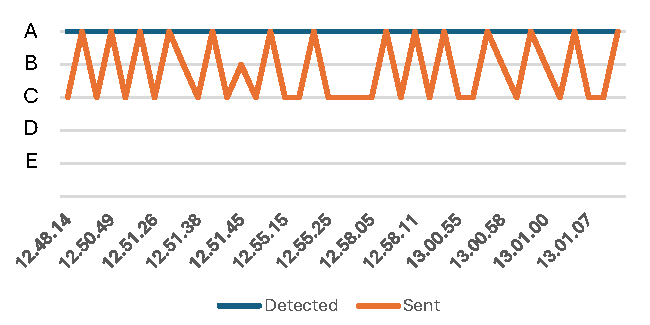
\includegraphics[width=1\textwidth]{gambar/tex/left.pdf}
    \caption{Left Turn Plots}
    \label{fig:left_turn_plots}
\end{figure}

Visualisasi pada gambar \ref{fig:left_turn_plots} berperan penting dalam mendeteksi adanya anomali atau kesalahan yang mungkin terjadi selama proses pengujian. Data yang dipilih untuk divisualisasikan merupakan salah satu hasil terbaik dari serangkaian percobaan terpisah yang telah dilakukan. Hal ini menunjukkan bahwa data tersebut merepresentasikan kondisi sistem yang optimal dan relevan untuk dianalisis lebih lanjut.

\begin{table}[H]
    \centering
    \caption{Summary of Data During Left Turn}
    \label{tab:left_turn_data_transmission_detection}
    \begin{tabular}{|c|c|}
        \hline 
        \cellcolor[HTML]{000000} & \cellcolor[HTML]{C0C0C0} \textbf{Percentage}  \\ \hline
        \cellcolor[HTML]{C0C0C0} \textbf{Transmitted as \texttt{C}} & 10.5 \\ \hline
        \cellcolor[HTML]{C0C0C0} \textbf{Same Register}  & 6.7 \\ \hline
        \cellcolor[HTML]{C0C0C0} \textbf{Different Register}   & 2.0 \\ \hline
    \end{tabular}
\end{table}

Tabel \ref{tab:left_turn_data_transmission_detection} merangkum data transmisi dan deteksi selama belok kiri. Persentase data yang dikirim sebagai \texttt{C} adalah 10.5\%, yang menunjukkan bahwa sistem sering mengirim instruksi untuk berhenti. Persentase data di mana deteksi dan data yang dikirim sama adalah 6.7\%, yang menunjukkan bahwa sistem berjalan sesuai dengan deteksi yang dilakukan. Persentase data di mana deteksi dan data yang dikirim berbeda adalah 2.0\%, yang menunjukkan adanya galat atau kesalahan dalam sistem.

\newpage
\subsection{Percobaan Belok Kanan}
\label{subsec:percobaanbelokkanan}

Bagian ini membahas kemampuan sistem dalam mengikuti objek saat berbelok ke kanan, yang pada dasarnya serupa dengan kondisi belok kanan. Tantangan yang dihadapi adalah bagaimana sistem mempertahankan objek dalam frame sambil melakukan penyesuaian sudut belok yang diperlukan. Solusinya meliputi pemanfaatan fusi data dari YOLOv11 dan MediaPipe Pose, serta penerapan algoritma kontrol yang mampu melakukan koreksi arah tepat waktu, sehingga sistem dapat mengikuti objek yang berbelok ke kanan dengan stabil dan akurat.

\begin{table}[H]
    \centering
    \caption{Data Performa Belok (Kanan)}
    \label{tab:performa_belok_kanan}
    \begin{tabular}{|c|c|c|c|c|c|c|c|c|}
    \hline
    Waktu & Reg (s) & YOLO (m) & MP (m) & x (px) & Deteksi & Terkirim & Keterangan \\ \hline
    12:48:09 & 0.2960 & 2.4469 & 1.6214 & 765 & b'E\textbackslash n' & b'C\textbackslash n' & Turn Right \\ \hline
    12:50:51 & 0.4610 & 1.4219 & 1.0142 & 830 & b'E\textbackslash n' & b'C\textbackslash n' & Turn Right \\ \hline
    12:50:56 & 0.6617 & 2.0234 & 1.6721 & 801 & b'E\textbackslash n' & b'C\textbackslash n' & Turn Right \\ \hline
    12:50:07 & 0.3573 & 1.4291 & 1.4911 & 795 & b'E\textbackslash n' & b'B\textbackslash n' & Turn Right \\ \hline
    12:50:07 & 0.3236 & 1.4588 & 1.7653 & 820 & b'E\textbackslash n' & b'C\textbackslash n' & Turn Right \\ \hline
    12:50:57 & 0.2675 & 2.0939 & 1.4524 & 825 & b'E\textbackslash n' & b'E\textbackslash n' & Turn Right \\ \hline
    12:51:07 & 3.9922 & 1.7796 & 1.3830 & 896 & b'E\textbackslash n' & b'C\textbackslash n' & Turn Right \\ \hline
    12:51:07 & 0.3518 & 2.0345 & 1.5442 & 883 & b'E\textbackslash n' & b'E\textbackslash n' & Turn Right \\ \hline
    12:51:11 & 2.3641 & 1.5332 & 1.5242 & 850 & b'E\textbackslash n' & b'C\textbackslash n' & Turn Right \\ \hline
    12:51:11 & 0.2897 & 2.0453 & 1.7421 & 792 & b'E\textbackslash n' & b'E\textbackslash n' & Turn Right \\ \hline
    12:51:22 & 0.2721 & 2.6141 & 1.7926 & 769 & b'E\textbackslash n' & b'C\textbackslash n' & Turn Right \\ \hline
    12:51:22 & 0.2947 & 2.7330 & 1.5570 & 867 & b'E\textbackslash n' & b'E\textbackslash n' & Turn Right \\ \hline
    12:51:31 & 0.2615 & 2.5602 & 1.3594 & 879 & b'E\textbackslash n' & b'C\textbackslash n' & Turn Right \\ \hline
    12:51:31 & 0.2711 & 2.2042 & 1.3829 & 827 & b'E\textbackslash n' & b'E\textbackslash n' & Turn Right \\ \hline
    12:51:41 & 2.8133 & 1.7721 & 1.4401 & 766 & b'E\textbackslash n' & b'C\textbackslash n' & Turn Right \\ \hline
    12:51:47 & 0.3573 & 1.4291 & 1.4911 & 795 & b'E\textbackslash n' & b'B\textbackslash n' & Turn Right \\ \hline
    12:51:48 & 0.3236 & 1.4588 & 1.7653 & 820 & b'E\textbackslash n' & b'C\textbackslash n' & Turn Right \\ \hline
    12:51:48 & 0.2701 & 1.9485 & 1.6638 & 792 & b'E\textbackslash n' & b'E\textbackslash n' & Turn Right \\ \hline
    12:51:56 & 0.2506 & 1.9262 & 1.7147 & 880 & b'E\textbackslash n' & b'C\textbackslash n' & Turn Right \\ \hline
    12:51:56 & 0.2716 & 1.9759 & 1.6276 & 871 & b'E\textbackslash n' & b'E\textbackslash n' & Turn Right \\ \hline
    12:55:09 & 1.9217 & 1.5004 & 1.8914 & 861 & b'E\textbackslash n' & b'C\textbackslash n' & Turn Right \\ \hline
    12:55:10 & 0.3128 & 2.1414 & 1.8698 & 858 & b'E\textbackslash n' & b'C\textbackslash n' & Turn Right \\ \hline
    12:55:10 & 0.3967 & 2.7356 & 2.0821 & 856 & b'E\textbackslash n' & b'E\textbackslash n' & Turn Right \\ \hline
    12:58:04 & 0.3573 & 1.4291 & 1.4911 & 795 & b'E\textbackslash n' & b'B\textbackslash n' & Turn Right \\ \hline
    12:58:04 & 0.3236 & 1.4588 & 1.7653 & 820 & b'E\textbackslash n' & b'C\textbackslash n' & Turn Right \\ \hline
    12:58:05 & 0.3560 & 1.6768 & 1.8145 & 795 & b'E\textbackslash n' & b'E\textbackslash n' & Turn Right \\ \hline
    13:01:13 & 1.1224 & 1.8459 & 1.5848 & 850 & b'E\textbackslash n' & b'C\textbackslash n' & Turn Right \\ \hline
    13:01:13 & 0.2936 & 1.5942 & 1.0293 & 832 & b'E\textbackslash n' & b'E\textbackslash n' & Turn Right \\ \hline
    13:01:17 & 0.3835 & 1.1238 & 1.0723 & 862 & b'E\textbackslash n' & b'B\textbackslash n' & Turn Right \\ \hline
    13:01:18 & 0.3058 & 1.1253 & 1.0494 & 845 & b'E\textbackslash n' & b'C\textbackslash n' & Turn Right \\ \hline
\end{tabular}
\end{table}

Tabel \ref{tab:performa_belok_kanan} menunjukkan data performa sistem saat berbelok ke kanan. Data ini mencakup waktu deteksi, jarak deteksi dari YOLOv11 dan MediaPipe Pose, posisi objek dalam frame, hasil deteksi, instruksi yang dikirimkan, dan keterangan mengenai arah belok. Data ini memberikan gambaran kinerja sistem dalam mengikuti objek yang berbelok ke kanan, termasuk kecepatan respons, akurasi deteksi, dan ketepatan instruksi yang dikirimkan.

\begin{figure}[H]
    \centering
    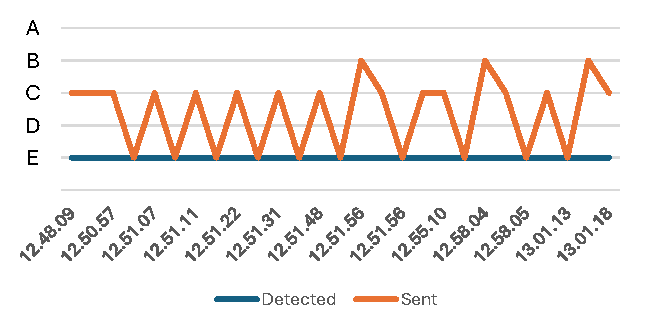
\includegraphics[width=1\textwidth]{gambar/tex/right.pdf}
    \caption{Right Turn Plots}
    \label{fig:right_turn_plots}
\end{figure}

Visualisasi pada gambar \ref{fig:right_turn_plots} berperan penting dalam mendeteksi adanya anomali atau kesalahan yang mungkin terjadi selama proses pengujian. Data yang dipilih untuk divisualisasikan merupakan salah satu hasil terbaik dari serangkaian percobaan terpisah yang telah dilakukan. Hal ini menunjukkan bahwa data tersebut merepresentasikan kondisi sistem yang optimal dan relevan untuk dianalisis lebih lanjut.

\begin{table}[H]
    \centering
    \caption{Summary of Data During Right Turn}
    \label{tab:right_turn_data_transmission_detection}
    \begin{tabular}{|c|c|}
        \hline 
        \cellcolor[HTML]{000000} & \cellcolor[HTML]{C0C0C0} \textbf{Percentage}   \\ \hline
        \cellcolor[HTML]{C0C0C0} \textbf{Transmitted as \texttt{C}} & 6.7  \\ \hline
        \cellcolor[HTML]{C0C0C0} \textbf{Same Register}  & 5.0  \\ \hline
        \cellcolor[HTML]{C0C0C0} \textbf{Different Register}   & 1.5  \\ \hline
    \end{tabular}
\end{table}

Tabel \ref{tab:right_turn_data_transmission_detection} merangkum data transmisi dan deteksi selama belok kanan. Persentase data yang dikirim sebagai \texttt{C} adalah 6.7\%, yang menunjukkan bahwa sistem sering mengirim instruksi untuk berhenti. Persentase data di mana deteksi dan data yang dikirim sama adalah 5.0\%, yang menunjukkan bahwa sistem berjalan sesuai dengan deteksi yang dilakukan. Persentase data di mana deteksi dan data yang dikirim berbeda adalah 1.5\%, yang menunjukkan adanya galat atau kesalahan dalam sistem.

\newpage
\subsection{Percobaan Luar Frame}
\label{subsec:percobaanluarframe}

Bagian ini membahas kemampuan sistem dalam menghadapi kondisi ketika objek keluar dari bidang pandang kamera (luar frame). Tantangan yang muncul adalah hilangnya data visual tentang posisi dan gerakan objek, sehingga sistem harus mampu memprediksi posisi berikutnya atau melakukan penyesuaian strategi pencarian. Solusi yang digunakan mencakup pengintegrasian algoritma prediksi lintasan serta inisialisasi ulang posisi, yang membantu sistem untuk kembali melacak objek setelah objek kembali ke dalam frame.

\begin{table}[H]
    \centering
    \caption{Data Status Frame (Luar Frame)}
    \label{tab:status_luar_frame}
    \begin{tabular}{|c|c|c|c|c|c|c|c|c|}
    \hline
    Waktu & Reg (s) & YOLO (m) & MP (m) & x (px) & Deteksi & Terkirim & Keterangan \\ \hline
    12:48:08 & 0.2758 & 0.0 & 0.0 & 0 & b'B\textbackslash n' & b'B\textbackslash n' & Forward \\ \hline
    12:48:08 & 0.3151 & 0.0 & 0.0 & 0 & b'B\textbackslash n' & b'B\textbackslash n' & Forward \\ \hline
    12:48:15 & 0.2931 & 0.0 & 0.0 & 0 & b'A\textbackslash n' & b'A\textbackslash n' & Turn Left \\ \hline
    12:48:18 & 0.3001 & 0.0 & 0.0 & 0 & b'B\textbackslash n' & b'B\textbackslash n' & Forward \\ \hline
    12:50:43 & 0.7366 & 0.0 & 0.0 & 0 & b'C\textbackslash n' & b'C\textbackslash n' & Stop \\ \hline
    12:50:43 & 0.3732 & 0.0 & 0.0 & 0 & b'C\textbackslash n' & b'C\textbackslash n' & Stop \\ \hline
    12:50:43 & 0.2571 & 0.0 & 0.0 & 0 & b'C\textbackslash n' & b'C\textbackslash n' & Stop \\ \hline
    12:50:44 & 0.2395 & 0.0 & 0.0 & 0 & b'E\textbackslash n' & b'E\textbackslash n' & Turn Right \\ \hline
    12:50:44 & 0.3522 & 0.0 & 0.0 & 0 & b'C\textbackslash n' & b'C\textbackslash n' & Stop \\ \hline
    12:50:44 & 0.3647 & 0.0 & 0.0 & 0 & b'C\textbackslash n' & b'C\textbackslash n' & Stop \\ \hline
    12:50:45 & 0.3504 & 0.0 & 0.0 & 0 & b'C\textbackslash n' & b'C\textbackslash n' & Stop \\ \hline
    12:50:49 & 0.3535 & 0.0 & 0.0 & 0 & b'A\textbackslash n' & b'A\textbackslash n' & Turn Left \\ \hline
    12:51:07 & 0.3518 & 0.0 & 0.0 & 0 & b'E\textbackslash n' & b'E\textbackslash n' & Turn Right \\ \hline
    12:51:11 & 0.2897 & 0.0 & 0.0 & 0 & b'E\textbackslash n' & b'E\textbackslash n' & Turn Right \\ \hline
    12:51:26 & 0.3185 & 0.0 & 0.0 & 0 & b'B\textbackslash n' & b'B\textbackslash n' & Forward \\ \hline
    12:51:30 & 0.2687 & 0.0 & 0.0 & 0 & b'B\textbackslash n' & b'B\textbackslash n' & Forward \\ \hline
    12:51:31 & 0.2615 & 0.0 & 0.0 & 0 & b'E\textbackslash n' & b'E\textbackslash n' & Turn Right \\ \hline
    12:51:31 & 0.2711 & 0.0 & 0.0 & 0 & b'E\textbackslash n' & b'E\textbackslash n' & Turn Right \\ \hline
    12:51:38 & 0.2502 & 0.0 & 0.0 & 0 & b'A\textbackslash n' & b'A\textbackslash n' & Turn Left \\ \hline
    12:51:38 & 0.2617 & 0.0 & 0.0 & 0 & b'A\textbackslash n' & b'A\textbackslash n' & Turn Left \\ \hline
    12:52:05 & 0.6562 & 0.0 & 0.0 & 0 & b'B\textbackslash n' & b'B\textbackslash n' & Forward \\ \hline
    12:58:09 & 0.3319 & 0.0 & 0.0 & 0 & b'B\textbackslash n' & b'B\textbackslash n' & Forward \\ \hline
    12:58:11 & 0.2506 & 0.0 & 0.0 & 0 & b'A\textbackslash n' & b'A\textbackslash n' & Turn Left \\ \hline
    13:00:57 & 0.3574 & 0.0 & 0.0 & 0 & b'C\textbackslash n' & b'C\textbackslash n' & Stop \\ \hline
    13:01:07 & 0.2856 & 0.0 & 0.0 & 0 & b'A\textbackslash n' & b'A\textbackslash n' & Turn Left \\ \hline
    13:01:12 & 0.2639 & 0.0 & 0.0 & 0 & b'B\textbackslash n' & b'B\textbackslash n' & Forward \\ \hline
    13:01:16 & 1.3214 & 0.0 & 0.0 & 0 & b'C\textbackslash n' & b'C\textbackslash n' & Stop \\ \hline
    13:01:16 & 0.3159 & 0.0 & 0.0 & 0 & b'C\textbackslash n' & b'C\textbackslash n' & Stop \\ \hline
    13:01:17 & 0.3360 & 0.0 & 0.0 & 0 & b'C\textbackslash n' & b'C\textbackslash n' & Stop \\ \hline
    13:01:19 & 0.2638 & 0.0 & 0.0 & 0 & b'C\textbackslash n' & b'C\textbackslash n' & Stop \\ \hline
    \end{tabular}
\end{table}
Tabel \ref{tab:status_luar_frame} menunjukkan data status sistem saat objek berada di luar frame. Data ini memperlihatkan saat nilai dari deteksi objek keduanya adalah 0 dan keterangan mengenai status objek. Data ini memberikan gambaran kinerja sistem dalam menghadapi kondisi ketika objek keluar dari bidang pandang kamera, termasuk kecepatan respons, akurasi deteksi, dan ketepatan instruksi yang dikirimkan.

Beberapa data telah difilter untuk menampilkan data yang menunjukkan sistem bekerja dengan sempurna ketika tidak ada objek yang terdeteksi dan mengirimkan kode instruksi sebelumnya tanpa penundaan yang lama ke mesin. Namun, ada masalah serius di mana sistem terus-menerus mengirimkan kode instruksi maju tanpa jaminan bahwa objek akan terdeteksi untuk mengubah kode instruksi ke mesin. Hal ini dapat menyebabkan potensi risiko keselamatan dan ketidakefisienan dalam operasi sistem.

\section{Performa Keberhasilan Mengikuti}
\label{sec:performamengikuti}

Bagian ini menguji apakah sistem dapat mengikuti objek pada lajur khusus, seperti jalur sempit atau berbelok yang membutuhkan manuver khusus.

\section{Pembahasan Hasil}
\label{sec:pembahasanhasil}

Bagian ini membahas hasil-hasil pengujian secara keseluruhan dan memberikan insight mengenai performa sistem.

\subsection{Performa Deteksi Objek}
\label{sec:performadeteksiobjek}

Bagian ini menjelaskan kekuatan dan kelemahan deteksi objek yang ditemukan selama pengujian.

\subsection{Kecepatan Pemrosesan (FPS)}
\label{sec:kecepatanpemrosesan}

Menganalisis kecepatan pemrosesan secara keseluruhan dan pengaruhnya terhadap performa sistem real-time.

\subsection{Response Time}
\label{sec:responsetime}

Membahas hasil pengujian response time dan faktor-faktor yang mempengaruhi waktu respons.

\subsection{Keberhasilan Tracking}
\label{sec:performatracking}

Membahas tingkat keberhasilan sistem dalam melacak objek dan kondisi yang mempengaruhi performa.

\subsection{Kesesuaian Tingkat Pencahayaan}
\label{sec:kesesuaianpencahayaan}

Membahas tingkat keberhasilan sistem dalam melacak objek pada kondisi pencahayaan yang berbeda.

\subsection{Kesesuaian Jarak Deteksi}
\label{sec:kesesuaianjarak}

Diskusi tentang performa sistem dalam mendeteksi objek pada berbagai jarak yang telah diuji.

\subsection{Performa Pergerakan Mengikuti Objek}
\label{sec:akurasiikutiobjek}

Evaluasi akurasi dalam mengikuti objek target, termasuk kondisi yang dapat menyebabkan kegagalan.

\subsection{Performa Keberhasilan Mengikuti}
\label{sec:keberhasilanmengikuti}

Menguraikan keberhasilan sistem dalam mengikuti objek saat menghadapi belokan dan lajur khusus.